\documentclass{article}
\usepackage[utf8]{inputenc}
\usepackage{amsmath}
\usepackage{bm}
\usepackage{graphicx}
\graphicspath{ {./images/} }

\title{Kalman Filter}
\author{Alexandru Meterez}
\date{April 2020}

\begin{document}
\maketitle

\section{Introduction}
Kalman Filter works by combining two possible bad measurments on their own (with big errors) into a much better one:
\begin{itemize}
    \item the physical model of the system
    \item the measurements of the sensors
\end{itemize}
Let's take an example. Let's say we have a car and we want to know its position. For this we have 2 sensors, one that measures the \textbf{position} and one that measures the \textbf{speed}. Unfortunately, both of them have errors. However, we can incorporate the measurements with the physical model of the system $x_n = x_{n-1} + v_{n-1} \cdot \Delta t$ in order to minimise the error. In other words, we combine:
\begin{itemize}
    \item I know where I am know, my speed and the time and according to Newton, I'll be at some $x_n$ later
    \item I know that my sensor tells me that I will be at some other $x_n$
\end{itemize} 
Both of them are "wronger" on their own, then together. \\
A visual explanation is that it works based on overlapping Gaussians. You have a Gaussian around the estimate from the physical model and one around the measurement from the sensors (see figure \ref{fig1}). If you calculate the intersection (product of Gaussians), you get a smaller variance and thus a smaller error (see figure \ref{fig2}).
\begin{figure}[b]
    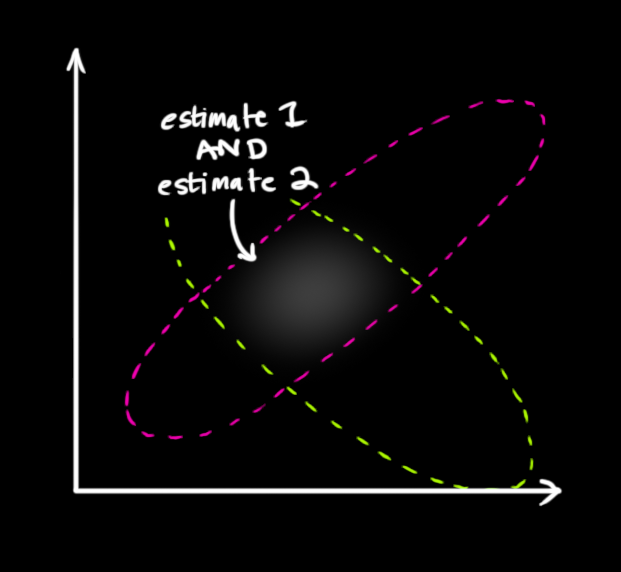
\includegraphics[width=0.75\textwidth]{pic2.png}
    \centering
    \caption{Overlapping Gaussians}
    \label{fig1}
\end{figure}
\begin{figure}[b]
    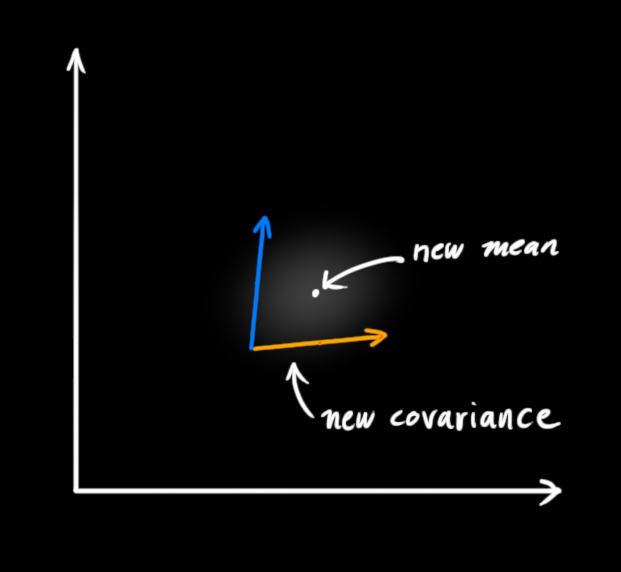
\includegraphics[width=0.75\textwidth]{pic3.png}
    \centering
    \caption{New variance}
    \label{fig2}
\end{figure}

\section{Algorithm}
The Kalman Filter algorithm is pretty easy and it consists of 2 major steps:
\begin{enumerate}
    \item \textbf{Predict} the state based on the physical system
    \item \textbf{Update} the prediction based on the measurement from the sensors
\end{enumerate}
We thus have an \textbf{iterative process}.

\section{1D Kalman Filter}

\textbf{Predict}
\begin{equation}
    \hat{x_k} = \hat{x_{k-1}} + \Delta t \cdot \hat{\dot{x_{k-1}}}
\end{equation}
\begin{equation}
    \hat{\dot{x_k}} = \hat{\dot{x_{k-1}}}
\end{equation}
\begin{equation}
    p_k = p_{k-1} + q
\end{equation}

\textbf{Update}
\begin{equation}
    K_k := p_k(p_k + r)^{-1}
\end{equation}
\begin{equation}
    \hat{x_k} := \hat{x_k} + K_k(z_k - \hat{x_k})
\end{equation}
\begin{equation}
    p_k := (1-K_k)p_k
\end{equation}
And now plugin $x_k$ and $p_k$ into the predict step again and iterate.\\
\textbf{Observation}: The equations (1) and (2) are not set in stone. This example is for the position of a moving object with constant velocity, that's why the rules look like this. Also, because I want them to look similar to the way they are written in the matrix form. But they can change based on what the system is doing. 

\begin{itemize}
    \item $x_k$ - position at time $k$
    \item $\dot{x_k}$ - velocity at time $k$
    \item $p_k$ - estimation error - how far our estimate is from the truth
    \item $q$ - process error - how far our physical model is from the truth (for example it doesn't include wind, or wheel friction and so on)
    \item $r$ - measurement error - how far our sensors are from the truth
    \item $K_k$ - Kalman gain - looks at how big the errors of the estimate and the measurement are in eq. (4) and then chooses how much to take into consideration (weighs) the measurement and the estimate in eq. (5)
    \item $z_k$ - measurement from sensors
\end{itemize}
This notation is cumbersome, especially if we want to have a stat with many more variables. We can go to the matrix form, by placing the position and speed in a vector and vectorize the equations.

\section{Matrix form Kalman Filter}
\textbf{Predict}
\begin{equation}
    \bm{\hat{x_k}} = F_k\bm{\hat{x_{k-1}}} + B_k\bm{u_k}
\end{equation}
\begin{equation}
    P_k = F_kP_{k-1}F_k^T + Q_k
\end{equation}
\textbf{Update}
\begin{equation}
    \bm{\hat{x_k}} := \bm{\hat{x_k}} + K_k(\bm{z_k}-H_k\bm{\hat{x_k}})
\end{equation}
\begin{equation}
    P_k := P_k - K_kH_kP_k
\end{equation}
\begin{equation}
    K_k = P_kH_K^T(H_kP_kH_k^T + R_k)^{-1}
\end{equation}

\begin{itemize}
    \item $\bm{x_k} = \begin{bmatrix}
        x_k \\
        \dot{x_k}
    \end{bmatrix}$ and is the state of the system
    \item $F$: state transition matrix
    \item $\bm{u}$: control variable - usually has the acceleration
    \item $B$: control matrix - maps control to state variables
    \item $P$: state covariance matrix - error of estimates
    \item $Q$: process covariance matrix - error due to process
    \item $\bm{z}$: measurement from sensors
    \item $H$: measurement matrix - maps measurements into state
    \item $K_k$: Kalman gain
    \item $R$: Measurement covariance matrix - error from measurements
\end{itemize}

\end{document}